\documentclass{article}
% \usepackage{ctex} % 思考1：将这行取消注释，看看会有什么不同

\usepackage{lipsum}

\usepackage{geometry}
\geometry{a4paper, margin=1in}

\usepackage{graphicx}
\graphicspath{{figures/}}   % 图片所在路径

\linespread{1.5}

% 思考2：注释下面4行（15-18行），看看会有什么不同
% % 去掉图编号与题注文字之间的冒号，改为两个空格
\usepackage{caption}
\DeclareCaptionLabelSeparator{twospace}{~~}
\captionsetup{labelsep=twospace}

\begin{document}

\lipsum[1]

As shown in Figure \ref{fig:starryNight}.
% 中文环境中，可采用下面这行代码
% 如图~\ref{fig:starryNight}~所示。

% 思考3：删除下面 figure 环境的位置参数 [htbp]，看看会发生什么
\begin{figure}[htbp]
    \centering
    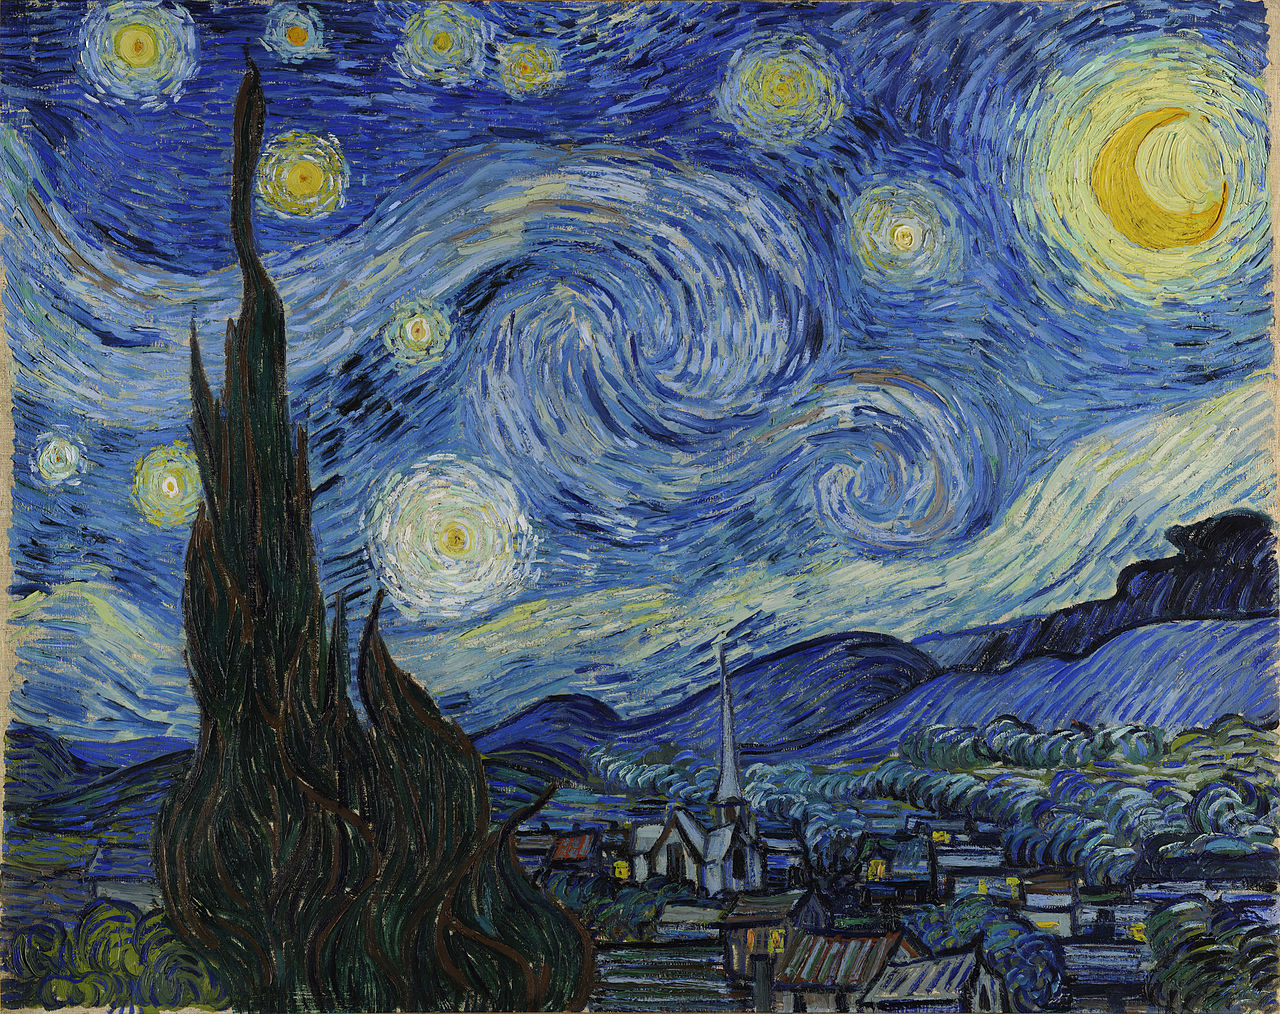
\includegraphics[width=0.6\linewidth]{starryNight.jpg}
    \caption{A figure of starry night by Vincent}
    \label{fig:starryNight}
\end{figure}

\lipsum[2]

\end{document}
